
%%%%%%%%%%%%%%%%%%%%%%%%%%%%%%%%%%%%%%%%%%%%%%%%%%%%%%%%%%%%%%%%%%%%%%%%%%%%%%
% Copyright (c) 2003-2015 by The University of Queensland
% http://www.uq.edu.au
%
% Primary Business: Queensland, Australia
% Licensed under the Open Software License version 3.0
% http://www.opensource.org/licenses/osl-3.0.php
%
% Development until 2012 by Earth Systems Science Computational Center (ESSCC)
% Development 2012-2013 by School of Earth Sciences
% Development from 2014 by Centre for Geoscience Computing (GeoComp)
%
%%%%%%%%%%%%%%%%%%%%%%%%%%%%%%%%%%%%%%%%%%%%%%%%%%%%%%%%%%%%%%%%%%%%%%%%%%%%%%

\section{Fault System}
\label{Fault System}
The \class{FaultSystem} class provides an easy-to-use interface to handle 2D
and 3D fault systems\index{faults} as used for instance in simulating fault
ruptures. The main purpose of the class is to provide a parameterization of
an individual fault in the system of faults.
In case of a 2D fault the fault is parameterized by a single value $w_{0}$ and
in the case of a 3D fault two parameters $w_{0}$ and $w_{1}$ are used.
This parameterization can be used to impose data (e.g. a slip distribution)
onto the fault. It can also be a useful tool to visualize or analyze the
results on the fault if the fault is not straight. 

\begin{figure}
\centering
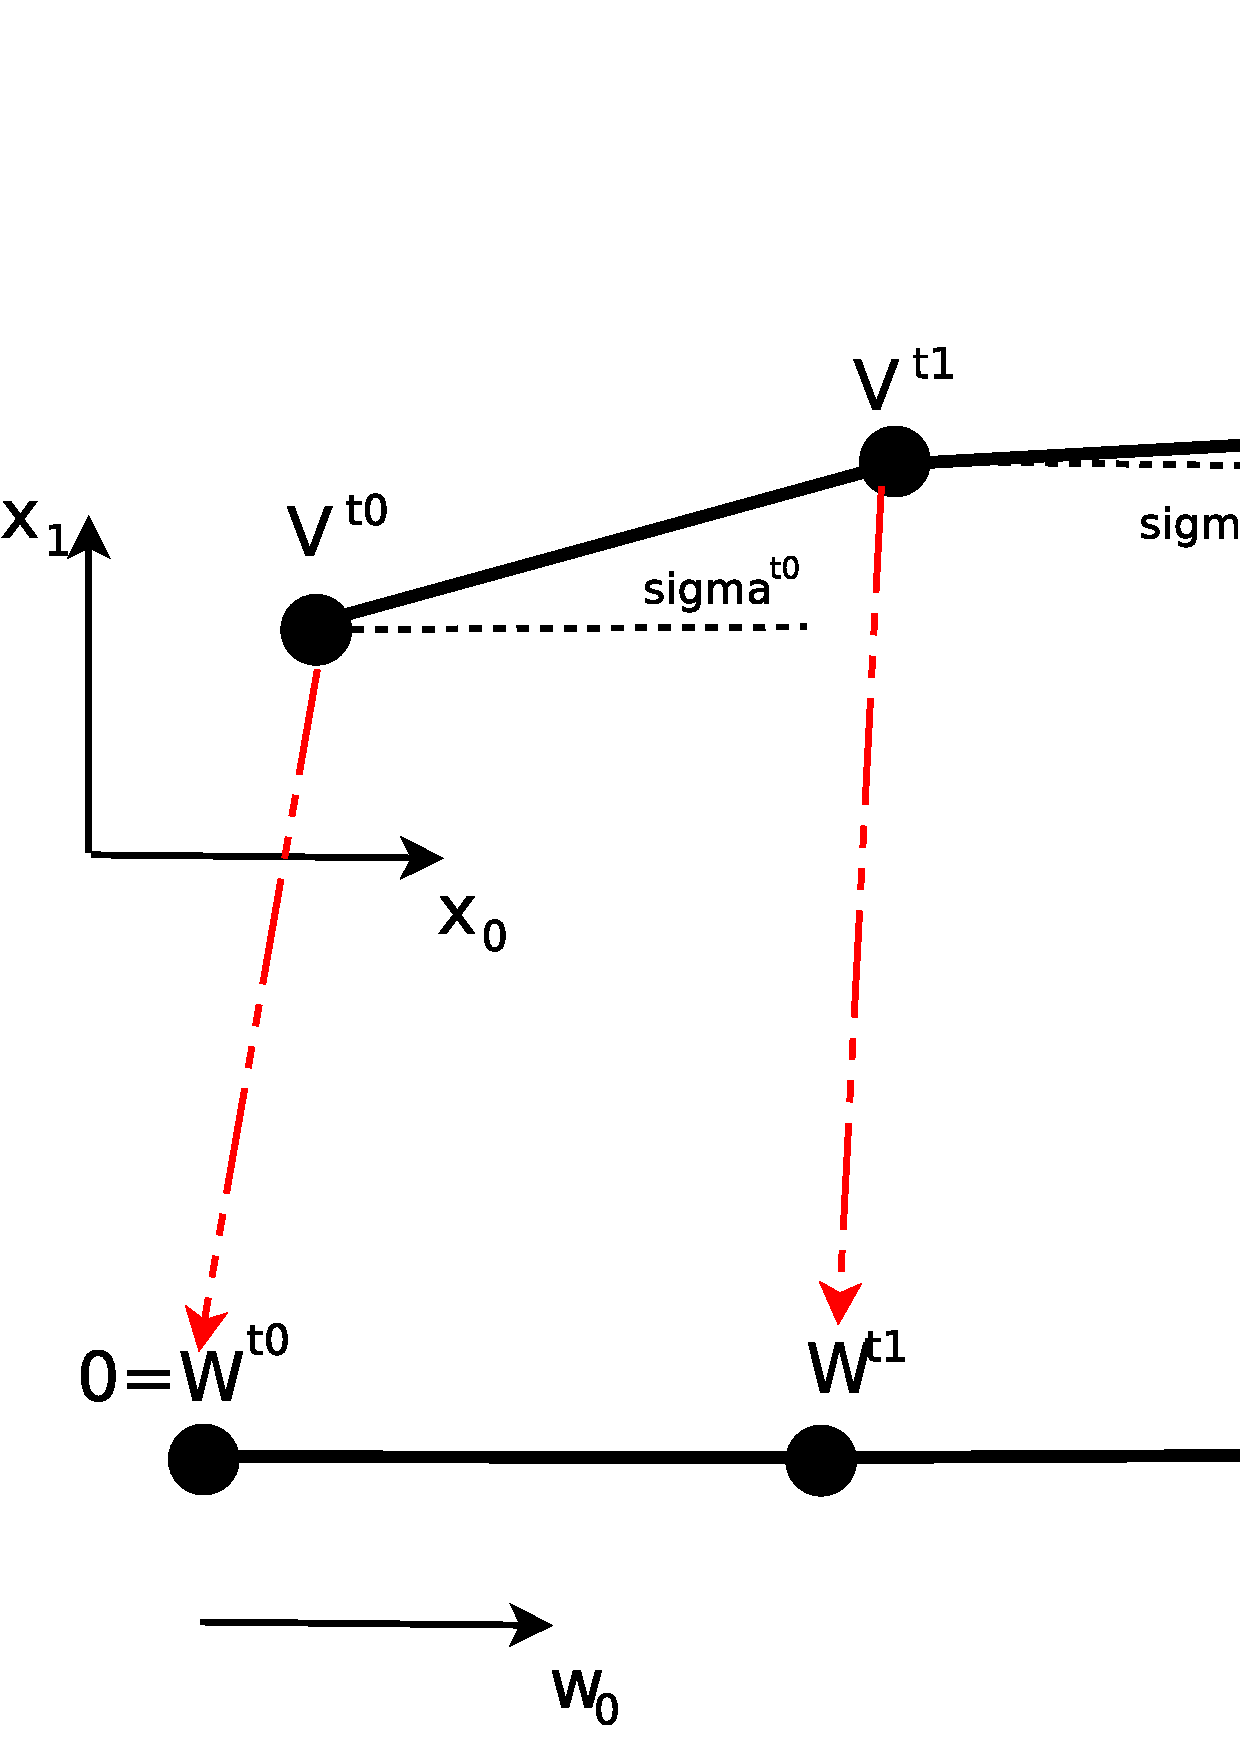
\includegraphics{FaultSystem2D}
\caption{\label{FAULTSYSTEM2D}Two dimensional fault system with one fault
named `t` in the $(x_{0},x_{1})$ space and its parameterization in the
$w_{0}$ space. The fault has three segments.}
\end{figure}

A fault $t$ in the fault system is represented by a starting point $V^{t0}$
and series of directions, called strikes\index{strike}, and the lengths $(l^{ti})$.
The strike of segment $i$ is defined by the angle $\sigma^{ti}$ between the
$x_{0}$-axis and the direction of the fault, see Figure~\ref{FAULTSYSTEM2D}.
The length and strike defines the polyline $(V^{ti})$ of the fault by
\begin{equation}
V^{ti} = V^{t(i-1)} + 
l^{ti} \cdot  S^{ti}
\mbox{ with }
S^{ti} =
\left[
\begin{array}{c}
 cos(\sigma^{ti})  \\
 sin(\sigma^{ti}) \\
 0 
\end{array}
\right]
\label{eq:fault 00}
\end{equation}
In the 3D case each fault segment $i$ has an additional dip\index{dip}
$\theta^{ti}$ and at each vertex $i$ a depth $\delta^{ti}$ is given.
The fault segment normal $n^{ti}$ is given by
\begin{equation}
n^{ti} = 
\left[
\begin{array}{c}
 -sin(\theta^{ti}) \cdot S^{ti}_{1} \\
 sin(\theta^{ti}) \cdot S^{ti}_{0} \\
 cos(\theta^{ti}) 
\end{array}
\right]
\label{eq:fault 0}
\end{equation}
At each vertex we define a depth vector $d^{ti}$ defined as the intersect of
the fault planes of segment $(i-1)$ and $i$ where for the first segment and
last segment the vector orthogonal to strike vector $S^{ti}$\index{strike}
and the segment normal $n^{ti}$ is used. The direction $\tilde{d}^{ti}$ of the
depth vector is given as
\begin{equation}
\tilde{d}^{ti} = n^{ti} \times n^{t(i-1)}
\label{eq:fault b}
\end{equation}
If $\tilde{d}^{ti}$ is zero the strike vectors $L^{t(i-1)}$ and $L^{ti}$ are
collinear and we can set $\tilde{d}^{ti} = l^{ti} \times n^{ti}$.
If the two fault segments are almost orthogonal $\tilde{d}^{ti}$ is pointing
in the direction of $L^{t(i-1)}$ and $L^{ti}$. In this case no depth can be
defined. So we will reject a fault system if
\begin{equation}
min(\| \tilde{d}^{ti}  \times  L^{t(i-1)} \|,\| \tilde{d}^{ti}  \times  L^{ti} \|) 
\le 0.1 \cdot \| \tilde{d}^{ti} | 
\label{eq:fault c}
\end{equation}
which corresponds to an angle of less than $10^o$ between the depth vector and
the strike. We then set
\begin{equation}
d^{ti}=\delta^{ti} \cdot \frac{\tilde{d}^{ti}}{\|\tilde{d}^{ti}\|}
\label{eq:fault d}
\end{equation}
We can then define the polyline $(v^{ti})$ for the bottom of the fault as
\begin{equation}
v^{ti}= V^{ti}+d^{ti}
\label{eq:fault e}
\end{equation}
In order to simplify working on a fault $t$ in a fault system a
parameterization $P^t: (w_{0},w_{1}) \rightarrow (x_{0},x_{1},x_{2})$ over a
rectangular domain is introduced such that
\begin{equation}
0\le w_{0} \le w^t_{0 max} \mbox{ and }  -w^t_{1max}\le w_{1} \le 0
\label{eq:fault 1}
\end{equation}
with positive numbers $w^t_{0 max}$ and $w^t_{1 max}$. Typically one chooses
$w^t_{0 max}$ to be the unrolled length of the fault and $w^t_{1 max}$ to be
the mean value of segment depth. Moreover we have
\begin{equation}
P^t(W^{ti})=V^{ti}\mbox{ and } P^t(w^{ti})=v^{ti}\
\label{eq:fault 2}
\end{equation}
where
\begin{equation}
W^{ti}=(\Omega^{ti},0) \mbox{ and } w^{ti}=(\Omega^{ti},-w^t_{1 max})
\label{eq:fault 3}
\end{equation}
and $\Omega^{ti}$ is the unrolled distance of $W^{ti}$ from $W^{t0}$, i.e.
$l^{ti}=\Omega^{t(i+1)}-\Omega^{ti}$. In the 2D case $w^t_{1 max}$ is set to
zero and therefore the second component is dropped, see Figure~\ref{FAULTSYSTEM2D}.

In the 2D case the parameterization $P^t$ is constructed as follows:
The line connecting $V^{t(i-1)}$ and $V^{ti}$ is given by
\begin{equation}
x=V^{ti} + s  \cdot  ( V^{t(i+1)}- V^{ti} )
\label{eq:2D line 1}
\end{equation}
where $s$ is between $0$ and $1$. The point $x$ is on $i$-th fault segment if
and only if such an $s$ exists. Assuming $x$ is on the fault it can be
calculated as
\begin{equation}
s = \frac{ (x- V^{ti})^t \cdot (V^{t(i+1)}- V^{ti}) }{ \|V^{t(i+1)}- V^{ti}\|^2} 
\label{eq:2D line 1b}
\end{equation}
We then can set
\begin{equation}
w_{0}=\Omega^{ti}+s \cdot (\Omega^{ti}-\Omega^{t(i-1)})
\label{eq:2D line 2}
\end{equation}
to get $P^t(w_{0})=x$.
It remains the question if the given $x$ is actually on the segment $i$ of
fault $t$. To test this $s$ is restricted between $0$ and $1$ (so if $s<0$, $s$
is set to $0$ and if $s>1$, $s$ is set to $1$) and then we check the residual
of \eqn{eq:2D line 1}, i.e. $x$ has been accepted to be in the segment if
\begin{equation}
\|x-V^{ti} - s \cdot (V^{t(i+1)}- V^{ti}) \| \le tol \cdot  
max(l^{ti}, \|x-V^{ti} \|) 
\label{eq:2D line 3}
\end{equation}
where $tol$ is a given tolerance.

In the 3D case the situation is a bit more complicated: we split the fault
segment across the diagonal $V^{ti}$-$v^{t(i+1)}$ to produce two triangles.
In the upper triangle we use the parameterization 
\begin{equation}
x= V^{ti} + s \cdot (V^{t(i+1)}-V^{ti})  + r \cdot (v^{t(i+1)}-V^{t(i+1)})
\mbox{ with } r \le s; 
\label{eq:2D line 4}
\end{equation}
while in the lower triangle we use
\begin{equation}
x= V^{ti} +  s \cdot (v^{t(i+1)}-v^{ti}) + r \cdot (v^{ti}-V^{ti})
\mbox{ with } s \le r; 
\label{eq:2D line 4b}
\end{equation}
where $0\le s,r \le 1$. Both equations are solved in the least-squares sense
e.g. using the Moore-Penrose pseudo-inverse for the coefficient matrices.
The resulting $s$ and $r$ are then restricted to the unit square. Similar to
the 2D case (see \eqn{eq:2D line 3}) we identify $x$ to be in the upper
triangle of the segment if
\begin{equation}
\|x- V^{ti} - s \cdot (V^{t(i+1)}-V^{ti})  - r \cdot (v^{t(i+1)}-V^{t(i+1)}) \|
\le tol \cdot  max(\|x-V^{ti} \|,\|v^{t(i+1)}-V^{t(i)})\|) 
\label{eq:2D line 4c}
\end{equation}
and in the lower part
\begin{equation}
\|x-V^{ti} -  s \cdot (v^{t(i+1)}-v^{ti}) - r \cdot (v^{ti}-V^{ti}) \|
\le tol \cdot  max(\|x-V^{ti} \|,\|v^{t(i+1)}-V^{t(i)})\|)  
\label{eq:2D line 4d}
\end{equation}
after the restriction of $(s,t)$ to the unit square.
Note that $\|v^{t(i+1)}-V^{t(i)})\|$ is the length of the diagonal of the
fault segment. For those $x$ which have been located in the $i$-th segment we
then set
\begin{equation}
w_{0}=\Omega^{ti}+s \cdot (\Omega^{ti}-\Omega^{t(i-1)})
\mbox{ and }
w_{1}=w^t_{1max} (r-1) 
\label{eq:2D line 5}
\end{equation}

\subsection{Functions}

\begin{classdesc}{FaultSystem}{\optional{dim =3}}
creates a fault system in the \var{dim} dimensional space.
\end{classdesc}

\begin{methoddesc}[FaultSystem]{getMediumDepth}{tag}
returns the medium depth of fault \var{tag}.
\end{methoddesc}

\begin{methoddesc}[FaultSystem]{getTags}{}
returns a list of the tags used by the fault system.
\end{methoddesc}

\begin{methoddesc}[FaultSystem]{getStart}{tag}
returns the starting point of fault \var{tag} as a \numpyNDA object.
\end{methoddesc}

\begin{methoddesc}[FaultSystem]{getDim}{}
returns the spatial dimension.
\end{methoddesc}

\begin{methoddesc}[FaultSystem]{getDepths}{tag}
returns the list of the depths of the segments in fault \var{tag}.
\end{methoddesc}

\begin{methoddesc}[FaultSystem]{getTopPolyline}{tag}
returns the polyline used to describe the fault tagged by \var{tag}.
\end{methoddesc}

\begin{methoddesc}[FaultSystem]{getStrikes}{tag}
returns the list of strikes $\sigma^{ti}$ of the segments in fault
$t=$\var{tag}.
\end{methoddesc}

\begin{methoddesc}[FaultSystem]{getStrikeVectors}{tag}
returns the strike vectors $S^{ti}$ of fault $t=$\var{tag}.
\end{methoddesc}

\begin{methoddesc}[FaultSystem]{getLengths}{tag}
returns the lengths $l^{ti}$ of the segments in fault $t=$\var{tag}.
\end{methoddesc}

\begin{methoddesc}[FaultSystem]{getTotalLength}{tag}
returns the total unrolled length of fault \var{tag}.
\end{methoddesc}

\begin{methoddesc}[FaultSystem]{getDips}{tag}
returns the list of the dips of the segments in fault \var{tag}.
\end{methoddesc}

\begin{methoddesc}[FaultSystem]{getBottomPolyline}{tag}
returns the list of the vertices defining the bottom of the fault \var{tag}.
\end{methoddesc}

\begin{methoddesc}[FaultSystem]{getSegmentNormals}{tag}
returns the list of the normals of the segments in fault \var{tag}.
\end{methoddesc}

\begin{methoddesc}[FaultSystem]{getDepthVectors}{tag}
returns the list of the depth vectors $d^{ti}$ for fault $t=$\var{tag}.
\end{methoddesc}

\begin{methoddesc}[FaultSystem]{getDepths}{tag}
returns the list of the depths of the segments in fault \var{tag}.
\end{methoddesc}

\begin{methoddesc}[FaultSystem]{getW0Range}{tag}
returns the range of the parameterization in $w_{0}$.
For tag $t$ this is the pair $(\Omega^{t0},\Omega^{tn})$ where $n$ is the
number of segments in the fault.
In most cases one has $(\Omega^{t0},\Omega^{tn})=(0,w^t_{0 max})$.
\end{methoddesc}

\begin{methoddesc}[FaultSystem]{getW1Range}{tag}
returns the range of the parameterization in  $w_{1}$.
For tag $t$ this is the pair $(-w^t_{1max},0)$.
\end{methoddesc}

\begin{methoddesc}[FaultSystem]{getW0Offsets}{tag}
returns the offsets for the parameterization of fault \var{tag}.
For tag \var{tag}=$t$ this is the list $[\Omega^{ti}]$.
\end{methoddesc}

\begin{methoddesc}[FaultSystem]{getCenterOnSurface}{}
returns the center point of the fault system at the surfaces.
In 3D the calculation of the center is considering the top edge of the faults
and projects the edge to the surface (the $x_{2}$ component is assumed to be
0). An \numpyNDA object is returned.
\end{methoddesc}

\begin{methoddesc}[FaultSystem]{getOrientationOnSurface}{}
returns the orientation of the fault system in RAD on the surface
($x_{2}=0$ plane) around the fault system center.
\end{methoddesc}

\begin{methoddesc}[FaultSystem]{transform}{\optional{rot=0, \optional{shift=numpy.zeros((3,)}}}
applies a shift \var{shift} and a consecutive rotation in the $x_{2}=0$ plane.
\var{rot} is a float number and \var{shift} an \numpyNDA object.
\end{methoddesc}

\begin{methoddesc}[FaultSystem]{getMaxValue}{f\optional{, tol=1.e-8}}
returns the tag of the fault where \var{f} takes the maximum value and a
\class{Locator} object which can be used to collect values from \Data objects
at the location where the maximum is taken, e.g.
\begin{python}
       fs=FaultSystem()
       f=Scalar(..)
       t, loc=fs.getMaxValue(f)
       print("maximum value of f on the fault %s is %s at location %s."%(t, \
             loc(f), loc.getX()))
\end{python}
\var{f} must be a \Scalar. When the maximum is calculated only
\DataSamplePoints are considered which are on a fault in the fault system in
the sense of condition~\ref{eq:2D line 3} or \ref{eq:2D line 4d}, respectively.
In the case no \DataSamplePoints are found the returned tag is \var{None} and
the maximum value as well as the location of the maximum value are undefined.
\end{methoddesc}

\begin{methoddesc}[FaultSystem]{getMinValue}{f\optional{, tol=1.e-8}}
returns the tag of the fault where \var{f} takes the minimum value and a
\class{Locator} object which can be used to collect values from \Data objects
at the location where the minimum is taken, e.g.
\begin{python}
  fs=FaultSystem()
  f=Scalar(..)
  t, loc=fs.getMinValue(f)
  print("minimum value of f on the fault %s is %s at location."%(t,loc(f),loc.getX()))
\end{python}
\var{f} must be a \Scalar. When the minimum is calculated only
\DataSamplePoints are considered which are on a fault in the fault system in
the sense of condition~\ref{eq:2D line 3} or \ref{eq:2D line 4d}, respectively.
In the case no \DataSamplePoints are found the returned tag is \var{None} and
the minimum value as well as the location of the minimum value are undefined.
\end{methoddesc}

\begin{methoddesc}[FaultSystem]{getParametrization}{x,tag \optional{\optional{, tol=1.e-8}, outsider=None}}
returns the argument $w$ of the parameterization $P^t$ for \var{tag}=$t$ to
provide \var{x} together with a mask indicating where the given location if on
a fault in the fault system by the value $1$ (otherwise the value is set to $0$).
\var{x} needs to be a \Vector or \numpyNDA object.
\var{tol} defines the tolerance to decide if given \DataSamplePoints are on
fault \var{tag}. The value \var{outside} is the value used as a replacement
value for $w$ where the corresponding value in \var{x} is not on a fault.
If \var{outside} is not present an appropriate value is used.
\end{methoddesc}
 
\begin{methoddesc}[FaultSystem]{getSideAndDistance}{x,tag}
returns the side and the distance at locations \var{x} from the fault \var{tag}.
\var{x} needs to be a \Vector or \numpyNDA object.
Positive values for side means that the corresponding location is to the right
of the fault, a negative value means that the corresponding location is
to the left of the fault. The value zero means that the side is undefined.
\end{methoddesc}

\begin{methoddesc}[FaultSystem]{getFaultSegments}{tag}
returns the polylines used to describe fault \var{tag}. For \var{tag}=$t$ this
is the list of the vertices $[V^{ti}]$ for the 2D and the pair of lists of the
top vertices $[V^{ti}]$ and the bottom vertices $[v^{ti}]$ in 3D.
Note that the coordinates are represented as \numpyNDA objects.
\end{methoddesc}

\begin{methoddesc}[FaultSystem]{addFault}{
strikes\optional{,
ls\optional{,
V0=[0.,0.,0.]\optional{,
tag=None\optional{,
dips=None\optional{,
depths= None\optional{,
w0_offsets=None\optional{,
w1_max=None}}}}}}}}
adds the fault \var{tag} to the fault system.
\var{V0} defines the start point of fault named $t=$\var{tag}.
The polyline defining the fault segments on the surface are set by the strike
angles \var{strikes} (=$\sigma^{ti}$, north = $\pi/2$, the orientation is
counterclockwise.) and the length \var{ls} (=$l^{ti}$).
In the 3D case one also needs to define the dip angles \var{dips}
(=$\delta^{ti}$, vertical=$0$, right-hand rule applies.) and the depth
\var{depths} for each segment.
\var{w1_max} defines the range of $w_{1}$.
If not present the mean value over the depth of all segment edges in the fault
is used.
\var{w0_offsets} sets the offsets $\Omega^{ti}$. If not present it is chosen
such that $\Omega^{ti}-\Omega^{t(i-1)}$ is the length of the $i$-th segment.
In some cases, e.g. when kinks in the fault are relevant, it can be useful
to explicitly specify the offsets in order to simplify the assignment of values.
\end{methoddesc}

\subsection{Example}
See \Sec{Slip CHAP}.

